\documentclass[12pt,a4paper]{report}

\usepackage{amsmath}
\usepackage{amsfonts}
%\usepackage{amssymb}
\usepackage{graphicx}
\usepackage{float}
\usepackage[autostyle]{csquotes}
\usepackage{acronym}
\usepackage{babel}
\usepackage{url}
\usepackage{algorithm}
\usepackage[noend]{algpseudocode}
\usepackage{tikz}
\usepackage{tabularx}
\usepackage{array}
%\usepackage{subfig}
\usepackage{titlesec}
\usepackage{caption}
\usepackage{subcaption}
\usepackage{mdframed}
\usepackage[legacy]{csvsimple}
\usepackage{siunitx}
\usepackage{url}

\usepackage[left=2cm,right=2cm,top=2.5cm,bottom=2.5cm]{geometry}

\usepackage[style=nature]{biblatex}
\addbibresource{sources.bib}

\newcolumntype{L}{>{\raggedright\arraybackslash}p}
\newcommand{\re}[1]{\textbf{\textcolor{orange}{#1}}}
\newcommand{\add}[1]{\textbf{\textcolor{blue}{#1}}}

\DeclareMathOperator*{\argmax}{argmax}

%\titleformat{\chapter}[display]
%{\normalfont\bfseries}{}{0pt}{\Large}


\title{
	A Sociable Virus? \\
	A Comparison and Investigation of Reproducibility of Methods for Analysing COVID-19 Transmission Chains Using Graph Networks
}


\author{Simon Westfechtel}

\begin{document}
	\emergencystretch 3em
	%\maketitle
	\begin{titlepage}
		\begin{center}
			\vspace*{1cm}
			
			\Huge
			\textbf{A Sociable Virus?}
			
			\vspace{0.5cm}
			\LARGE
			A Comparison and Investigation of Reproducibility of Methods for Analysing COVID-19 Transmission Chains Using Graph Networks
			
			\vspace{1cm}
			\large
			\textcolor{gray}{\textbf{Ein geselliges Virus?}}
			
			\vspace{0.5cm}
			\normalsize
			\textcolor{gray}{Ein Vergleich und eine Untersuchung der Reproduzierbarkeit von Methoden zur Analyse von COVID-19 Übertragungsketten mit Graphnetzwerken}
			
			\vfill
			
			\LARGE
			Master Thesis
			
			\large
			\textcolor{gray}{Masterarbeit}
			
			\vspace{0.4cm}
			
			\LARGE
			Computational Social Systems
			
			\vspace{0.8cm}
			
			\large
			Simon Westfechtel\\
			Matr.-Nr. 353822\\
			Aachen, \today
			\vfill
			
			\Large
			RWTH Aachen University\\
			Chair for Computational Social Sciences and Humanities\\
			
			\vfill
			\begin{flushleft}
				\normalsize
				Primary Supervisor / Erstprüfer: Priv.-Doz. Dr. Jürgen Lerner\\
				Secondary Supervisor / Zweitprüferin: Dr. Nazmiye Gizem Bacaksizlar Turbic\\
			\end{flushleft}
			
		\end{center}
	\end{titlepage}
	\begin{abstract}
		Scientific work on epidemics and pandemics mostly focuses on virology and potential treatments, while the societal aspect is often overlooked. The results are incoherent and often unfounded containment methods. The field of Computational Social Science offers a wide array of tools to analyse pandemic situations on a societal level. This work seeks to investigate and compare the usage of Social Network Analysis (SNA), Relational Event Models (REM) and Relational Hyperevent Models (RHEM) for this task. These methods are used to analyse six case contact networks from Europe and China. Results are compared to original reports where applicable to investigate reproducibility, and further compared horizontally (i.e. inter-regional) and vertically (i.e. inter-methodological). Results show a significant impact of age and sex on contact nomination likelihood, and a tendency for named contacts to become infected at later stages and interact with other contacts. Furthermore, Social Network Analysis and Relational (Hyper-)event Models should be used for different tasks. While no definitive answer can be given as to whether REM or RHEM are the preferable choice, findings justify the usage of RHEM over REM.  
	\end{abstract}
	\tableofcontents
	\chapter{Introduction}
\label{ch:Introduction}

When rumours of a novel respiratory virus, which would later be dubbed coronavirus disease 2019, or short COVID-19, first emerged from the People's Republic of China in late 2019, there was a lot of uncertainty regarding its danger potential. Authorities were hesitant to acknowledge the threat of a possible epidemic, and people were discouraged from stocking up on equipment such as protective face masks. When the virus spread to other countries across the globe and its impact could no longer be ignored, governments reversed course and imposed various restrictions on their respective populations, event going as far as sending a whole country into lockdown, in order to halt, or at least slow the spread of the virus. However, the sheer number of cases soon threatened to overwhelm healthcare systems worldwide.

In order to prevent this worst-case scenario, it became paramount to identify sources of infection and interrupt transmission chains. The efficient tracing of infected individuals' social contacts plays an integral part in preventing the spreading of a disease, and had been a well-established procedure well before the emergence of COVID-19, where for instance a verified case of tuberculosis requires a notification of the health departments \cite{enwiki_1097839709}. This is done to isolate persons who might have been infected by or have themselves been the source of infection of the individual, and therefore interrupt the transmission chain early, comparable to removing a domino piece to stop the fall of subsequent ones.

Most attention regarding science during the pandemic has focused on the medical field, especially the research of effective vaccines and treatments against the virus, but also virological factors (e.g. which individual features would predispose someone to infection and/or a severe course of illness, how the virus is transmitted from person to person, etc.). Now that the pandemic has mostly blown over, it has become apparent that there was a significant research gap regarding infection dynamics on a societal level, i.e. how the virus spread in social groups, as evident by arbitrary measures like curfews and restriction on social gatherings, the effectiveness of which have now been found to be questionable at best \add{CITE THIS}.

It is therefore necessary to establish a set of methods to effectively and efficiently analyse the social aspects of viral transmission and spread in order to be better prepared for a similar situation in the future. In the recent months, more work tackling this topic has emerged, and the field of computational social sciences offers a wide array of tools to address this problem.

Computational Social Science (CSS) is an interdisciplinary field that uses advanced computational methods to investigate social phenomena and human behavior. It combines elements of social sciences, such as sociology, economics, and psychology, with data science, computer science, and statistics. The aim is to glean insights into the complex dynamics of human societies through analysis of big data, modeling, and simulations, typically drawing from data sources like social media, web pages, or even administrative records.

The essence of CSS is the quantification and analysis of social phenomena, facilitating a deeper understanding of individual and group behaviors, social structures, and societal trends. By leveraging computational tools such as machine learning, network analysis, natural language processing, and agent-based modeling, CSS allows researchers to explore questions that were previously inaccessible due to the sheer complexity of the social systems involved. This often involves handling large and complex datasets, managing issues of privacy and ethics, and interpreting results in a meaningful social context.

\section{Contact tracing}
\label{sec:contact_tracing}

Many contact tracing initiatives were established during the course of the pandemic in most developed countries, e.g. automatic tracing via mobile apps; although they differ in the level of detail that was (or still is) being recorded, data collected at least included the source of infection, i.e. a symptomatic or, once tests had become widely available, positively tested patient, and said patient's social contacts, i.e. the people who had come into contact with them, and who thus could have been infected themselves and possibly spread the virus further. More rigorous systems also recorded covariates such as age, job or co-morbidities, which may play a role in transmission. 

A dataset consisting of records of the form (source, contact) can be modelled as a social network, a concept derived from graph theory, where individuals constitute a set of vertices, and contacts between individuals are represented by edges between the respective vertices; for an illustration, refer to figure \ref{fig:example_case_network}. These networks can be efficiently analysed using methods stemming from the field of computer science; thus, it becomes possible to identify dynamics in the spread of the virus on a social level, which are traditionally overlooked in virology. Common network effects include betweenness centrality, a measure for how instrumental a person is in facilitating the viral spread, or \add{which effect?} to determine whether infections emerge in clusters. Additionally, if further covariates like age, pre-existing illness or profession were also collected during the contact tracing procedure, methods from the field of data science can reliably discover patterns in the data and thus identify covariates that influence transmission, e.g. whether younger people are more likely to get infected and/or infect others compared to other age groups.

\begin{figure}
	\centering
	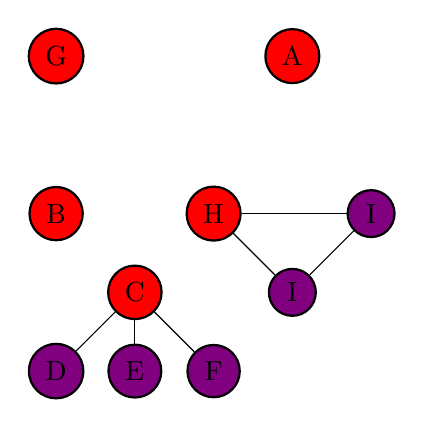
\begin{tikzpicture}
		\begin{scope}[every node/.style={circle,thick,draw,fill=red}]
			\node (A) at (2,2) {A};
			\node (B) at (-1,0) {B};
			\node (G) at (-1,2) {G};
			\node (C) at (0,-1) {C};
			\node (H) at (1,0) {H};
		\end{scope}
		
		\begin{scope}[every node/.style={circle,thick,draw,fill=violet}]
			\node (D) at (-1,-2) {D};
			\node (E) at (0,-2) {E};
			\node (F) at (1,-2) {F};
			\node (I) at (3,0) {I};
			\node (J) at (2,-1) {I};
		\end{scope}
		
		\begin{scope}
			\path (C) edge node {} (D);
			\path (C) edge node {} (E);
			\path (C) edge node {} (F);
			\path (H) edge node {} (I);
			\path (H) edge node {} (J);
			\path (I) edge node {} (J);
		\end{scope}
	\end{tikzpicture}
	\caption{Exemplary case contact network. Confirmed cases are coloured red, and reported contacts are coloured purple.}
	\label{fig:example_case_network}
\end{figure}

\section{Relational Event Models}
\label{sec:rem}

These static networks, however, can only give a partial representation of reality, since temporal information is omitted; thus, it is assumed that all infections and contact nominations happen simultaneously, whereas in reality, events occur sequentially. Therefore, infected patient $A$ might name person $B$ as a contact at time $t_1$, and $B$ might himself be recorded as a patient at a later time $t_2$, nominate persons $B,C,E$ as contacts, and so on. Obviously, this temporal aspect leads to a range of additional possible effects. Do dyads (pairs of source, contact) appear repeatedly (repetition), is a person $B$ who gets nominated as a contact by $A$ at time $t_n$ more likely to become a patient, and nominate $A$ in return at a later time $t_{n+m}$ (reciprocation), or is there a tendency for cyclic closure, where $A$ nominates $B$, $B$ then nominates $C$, and $C$ nominates $A$? \add{illustration}

A common method for modelling time-stamped relational data of the form (time, source, contact) are Relational Event Models, short REM, which were first proposed by \add{CITE}. They will be discussed further in chapter \ref{ch:methods}.

\section{Relational Hyperevent Models}
\label{sec:rhem}

An obvious shortcoming of relational event models is their dyadic nature, i.e. their inherent assumption that all interactions only involve two people at a time. Of course, this is not an accurate representation of reality. Think, for example, of John sending an email addressed at multiple of his colleagues, or in the context of COVID, Jane testing positive after attending a party and naming all the other guests as contacts. Some workarounds have been proposed to tackle this problem, like treating all interactions separately, or grouping all receiver nodes (email recipients and party attendees in our examples, respectively) into a single node. Refer to figure \ref{fig:polyadic_interactions} for an illustration. The problem with the former method is the fact that is treats the interactions as independent, while the latter may be unfeasible or even intractable for large datasets.

\begin{figure}
	\hspace*{\fill}
	\subfloat[Method 1: Model receiver set as a single node.]{
		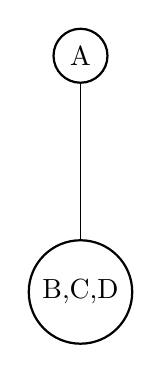
\begin{tikzpicture}
			\begin{scope}[every node/.style={circle,thick,draw}]
				\node (A) at (0,0) {A};
				\node (B) at (0,-3) {B,C,D};
			\end{scope}
			
			\begin{scope}
				\path (A) edge node {} (B);
			\end{scope}
		\end{tikzpicture}
	}
	\hfill
	\subfloat[Method 2: Model one edge for each node of the receiver set. Edges are assumed to be independent.]{
		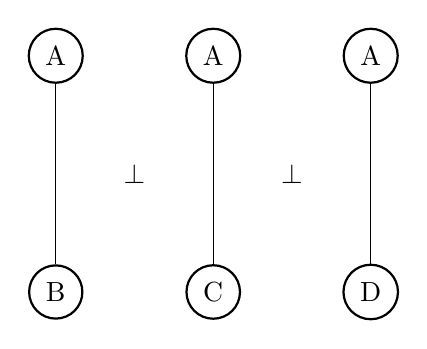
\begin{tikzpicture}
			\begin{scope}[every node/.style={circle,thick,draw}]
				\node (A1) at (0,0) {A};
				\node (A2) at (2,0) {A};
				\node (A3) at (4,0) {A};
				\node (B) at (0,-3) {B};
				\node (C) at (2,-3) {C};
				\node (D) at (4,-3) {D};
			\end{scope}
			
			\begin{scope}
				\node[draw=none] (A1A2) at (1,0) {};
				\node[draw=none] (BC) at (1,-3) {};
				\node[draw=none] (A2A3) at (3,0) {};
				\node[draw=none] (CD) at (3,-3) {};
			\end{scope}
			
			\begin{scope}
				\path (A1) edge node {} (B);
				\path (A2) edge node {} (C);
				\path (A3) edge node {} (D);
				\path (A1A2) edge[draw=none] node {$\perp$} (BC);
				\path (A2A3) edge[draw=none] node {$\perp$} (CD);
			\end{scope}
		\end{tikzpicture}
	}
	\hspace*{\fill}
	\caption{Two ways to approximate polydiadic interactions. In this example, A has an interaction with B, C, and D at the same time (e.g. They meet for a drink at the pub and A subsequently falls ill with Coronavirus).}
	\label{fig:polyadic_interactions}
\end{figure}

To address these issues, an extension to REM, named Relational Hyperevent Models, short RHEM, has been proposed by \add{CITE}. These models use hyperedges instead of the regular, dyadic edges known from graph theory; each hyperedge consists of a sender (e.g. a positively tested patient) and a set of receivers (e.g. attendees of a birthday party). These models can be used to discover effects in a fashion similar to REM, but with additional effects like partial repetition, where the receiver set is only partially the same in a repeated interaction (e.g. John plays tennis with Jane and Max, gets ill and nominates Max and Jane at time $t_n$, and again gets sick after grabbing coffee with Jane and Peter at time $t_{n+m}$ and thereafter nominates them), or unordered repetition, where an interaction is repeated involving the same actors, but the direction is not the same (e.g. reaching back to the previous example, John, Jane and Max again meet for tennis, whereafter Jane tests positive and nominates John and Max as contacts at time $t_{n+m}$). These RHEM will likewise be discussed in chapter \ref{ch:methods} in more detail.
	\chapter{Previous Work and Data Exploration}
\label{ch:previous_work_data}

This work seeks to compare methods proposed and corresponding results presented by Yang et al \cite{shaanxi_publication,hainan_publication} and Hâncean et al \cite{hancean2022occupations}. As alluded to in chapter \ref{ch:Introduction}, static network modelling, relational event modelling and relational hyperevent modelling will be compared against each other. These three methods will be applied to five different datasets. One is from Bucharest, Romania, which has already been analysed using relational hyperevent models by Hâncean et al \cite{hancean2022occupations}; three are from Yunnan, Hainan and Shanxi, China, which have all been analysed using static network models by Yang et al \cite{hainan_publication,shaanxi_publication}; the final dataset comprises records from all of China, and has, to the knowledge of the author, not been analysed at the time of writing this.

All the Chinese datasets are structures in the same basic manner, where records name the person who is being registered as a positively tested case, henceforth also referred to as referee; the person who is being nominated as a contact (if any), henceforth also referred to as referral; as well as covariates for referee and referral. Thus, one row equals one case contact nomination. Refer to table \ref{tab:china_data_structure} for an example. For these datasets, referees and referrals have all been tested positive for the virus.

The Romanian dataset, in contrast, consists of two tables, where one table contains all contact nominations akin to the Chinese ones, and one table contains information on positively tested patients. The patient information table contains all referees, but not all referrals, meaning that not all registered individuals were tested positive. 
To express this formally, let $A$ be the set of referees, $B$ be the set of referrals, and $P$ be the set of positively tested patients. For the Yunnan, Hainan, Shanxi and China dataset, it is $P = A \cup B$; for the Bucharest dataset, it is $A \subset P$, $B \not\subset P$, $P = A \cup X$, where $X = B_1 \cup B_2; B_1 \subset P, B_2 \not\subset P$.

\begin{table}
	\begin{tabularx}{\linewidth}{XXXXX}
		\hline
		\textbf{Timestamp} & \textbf{Referee} & \textbf{Referral} & \textbf{Referee covars [...]} & \textbf{Referral covars [...]} \\
		\hline
		2020-06-01 & p10 & p14 & ... & ... \\
		2020-06-01 & p10 & p17 & ... & ... \\
		2020-06-03 & p12 & - & ... & ... \\
		$\cdots$ & & & & \\
	\end{tabularx}
	\caption{General structure of the Chinese datasets. One row is equal to one contact nomination. Rows where the referral is empty mean there was no person nominated as contact by the referee. In this example, patient p10 nominated persons p14 and p17 as contacts, who themselves have also been tested positive. Patient p12, meanwhile, has not named anyone as a social contact.}
	\label{tab:china_data_structure}
\end{table}

\section{Yunnan Dataset}
\label{sec:yunnan_data}

\paragraph{Dataset overview} This dataset contains COVID case information from the province of Yunnan in southern China \cite{hainan_data}. There are 171 entries, with dates ranging from 2020-01-17 to 2020-02-16, i.e. this dataset is from the very early stages of the pandemic. The patient covariates deemed to be relevant are age, gender, and whether they are relatives of other confirmed cases listed in the dataset. All covariates are also listed in table \ref{tab:yunnan_hainan_covariates}.

\begin{table}
	\begin{minipage}{.45\linewidth}
		\begin{tabularx}{\linewidth}{L{.4\linewidth}L{.6\linewidth}}
			\hline
			\textbf{Covariate} & \textbf{Description}\\
			\hline
			Date & Date when the case was confirmed/reported\\
			Gender & Male/Female\\
			Age & In years\\
			Relatives & Whether the patient is a relative of previously recorded cases\\
			\hline
		\end{tabularx}
		\caption{Relevant covariates for the Yunnan and Hainan datasets}
		\label{tab:yunnan_hainan_covariates}
	\end{minipage}
	\hfill
	\begin{minipage}{.45\linewidth}
		\begin{tabularx}{\linewidth}{L{.4\linewidth}L{.6\linewidth}}
			\hline
			\textbf{Covariate} & \textbf{Description}\\
			\hline
			Date & Date when the case was confirmed/reported\\
			Gender & Male/Female\\
			Age & In years\\
			Hukou & Place of residence\\
			Relatives & Whether the patient is a relative of previously recorded cases\\
			\hline
		\end{tabularx}
		\caption{Relevant covariates for the Shanxi dataset}
		\label{tab:shanxi_covariates}
	\end{minipage}
	\begin{tabularx}{\linewidth}{L{.4\linewidth}L{.6\linewidth}}
		\hline
		\textbf{Covariate} & \textbf{Description}\\
		\hline
		Date & Date when the case was confirmed/reported\\
		Gender & Male/Female\\
		Age & In years\\
		Place of residence & \\
		Place and event & Activity where infection might have happened\\
		Symptom & The patient's symptoms\\
		Symptom severity & \\
		Place of admission & Where the patient was recorded by health authorities \\
		\hline
	\end{tabularx}
	\caption{Relevant covariates for the China dataset}
	\label{tab:china_covariates}
	\begin{tabularx}{\linewidth}{XXXXXX}
		\hline
		\textbf{Dataset} & \textbf{Age} & \textbf{Gender} & \textbf{Residence} & \textbf{Relatives} & \textbf{Degree}\\
		\hline
		Yunnan & $41\pm18$ & $\approx$ & - & $0.51$ & $1.3\pm3.2$\\
		Hainan & $48\pm17$ & $\approx$ & - & $0.46$ & $1.5\pm1.8$\\
		Shanxi & $46\pm16$ & $>men$ & Xian & $0.37$ & $0.99\pm1.3$\\
		China & $42\pm18$ & $>men$ & Xian & - & $3.6\pm18$\\
		\hline
	\end{tabularx}
	\caption{Comparison of covariates between datasets (where applicable). \emph{Gender} states which sex is more common, or whether they are roughly equal. \emph{Residence} is the most common value. \emph{Relatives} specifies the ratio of cases where relatives were recorded previously.}
	\label{tab:cov_comp}
\end{table}

Of the 171 individuals who have been confirmed positive, 114 cases have named no contacts at all, 25 have named one contact, eleven have named two contacts, and 21 have named three contacts or more. 58 and 62 cases are female and male, respectively; this information has not been recorded for the remaining 51 patients. This suggests neither sex is more susceptible to the virus. The average age of patients is $41\pm18$, with a 25 percentile of 26 and a 75 percentile of 54, meaning patients are mostly younger or middle-aged. From the 60 cases where this information is available, 31 are family members of other patients present in the dataset. 

\paragraph{Network analysis}
As previously mentioned, this dataset was analysed by Yang et al using network modelling \cite{hainan_publication}. In their work, they determined the effect of the aforementioned patient covariates like age and gender, as well as the following network effects:
\begin{itemize}
	\item degree centrality: a node-specific centrality measure, which is equal to the number of edges connected to a node $i$. Higher-degree nodes are therefore deemed more central, i.e. important, in the network \cite{golbeck}. In the context of case contact networks, these are the patients who nominate more contacts than average.
	\item betweenness centrality: a node-specific centrality measure, which for three nodes $i,j,k$ measures the ratio of the number of shortest paths from $j$ to $k$ that go through $i$ to the total number of shortest paths from $j$ to $k$. Nodes with a high betweenness centrality are nodes that facilitate the flow of information in the network, and are therefore deemed more central, i.e. important \cite{golbeck}. In the context of case context networks, these are the patients who are likely to have transmitted the virus from one cluster of patients to another.
	\item pagerank centrality: a node-specific centrality measure based on eigenvector centrality. It is computed by performing random walks on the network and measuring the likelihood to arrive at a node $p_i$ for all nodes. Nodes with a high pagerank centrality are frequently pointed at, and are therefore deemed more central, i.e. important \cite{gleich_pagerank}. In the context of case contact networks, these are patients who have been nominated as contacts more often than average.
	\item component size: connected components are sets of nodes in a network which are strongly connected, but have no outside connected, i.e. form a coherent and isolated community. In the context of case contact networks, these represent infection clusters, and the investigation of the size of these clusters can yield insights into how the virus tends to spread.
\end{itemize} They report an average degree centrality of $1.3\pm3.2$, an average betweenness centrality of $0\pm0$, and an average pagerank centrality of $0.0058\pm0.0055$. Furthermore, three of 18 connected components comprise of more than three nodes \cite{hainan_publication}. 

According to Yang et al, the zero value for betweenness centrality indicates that transmission of the virus from patient to patient happened near-simultaneously and in clusters, rather than in long transmission chains; A maximum pagerank score of 0.0221 compared to the mean value of $0.0058\pm0.0055$ means that ties are distributed unequally among patients, with a small number of patients being associated with most contact nominations. Furthermore, they write that the large fraction of nodes without ties is due to those patients hailing from another state, which made tracing of their contacts difficult; however, it isn't exactly stated why contact tracing was not possible for this group. The development of the case contact network over time was also analysed, albeit on a coarse level, where states of the network at three distinct points in time (start, middle and end point of the time period) were compared. Findings suggest that early cases were mostly imported from other provinces, since those mostly had no associated contacts, while local infection clusters only emerged in the later stages \cite{hainan_publication}. 

\section{Hainan Dataset}
\label{sec:hainan_data}

\paragraph{Dataset overview} This dataset contains COVID case information from the province of Hainan \cite{hainan_data}, which is the southernmost province of China. It was released in tandem with the Yunnan dataset, and therefore patient covariates are the same. There are 162 entries, with dates ranging from 2020-01-22 to 2020-02-14, i.e. this dataset is also from the early stages of the pandemic. Of the 162 confirmed cases, 71 have named no contacts, 27 have named one contact, 21 have named two contacts, and 43 have named three contacts or more. 

84 and 78 cases are female and male, respectively. An average age of $48\pm17$, a 25 percentile of 36 and a 75 percentile of 62 mean that the patients in this dataset are from an older age group compared to the Yunnan data. 75 out of 162 patients are family members of previously recorded cases.

\paragraph{Network analysis} This dataset was analysed by Yang et al using the same methodology outlined in section \ref{sec:yunnan_data}. They report an average degree centrality of $1.51\pm1.79$, an average betweenness centrality of $0\pm0$, and an average pagerank centrality of $0.0062\pm0.0043$. Ten out of 27 connected components are comprised of more than three nodes \cite{hainan_publication}. 

Interpretation of these numbers is similar to the Yunnan network. The zero value for betweenness centrality again indicated transmission happening in clusters rather than chains, and a maximum pagerank score of 0.0189 compared to the mean $0.0062\pm0.0043$ suggests an uneven distribution of ties. However, the larger fraction of patients with contacts (57\% here vs. just 33\% in the Yunnan dataset), paired with the larger number of connected components (27 vs. 18) means that less cases were imported from other states and/or containment measures might not have been as effective (the authors state that imposed measures were largely the same for both Yunnan and Hainan provinces). Accordingly, the temporal development of the case contact network shows an earlier emergence of infection clusters \cite{hainan_publication}.

\section{Shaanxi Dataset}
\label{sec:shaanxi_data}

\paragraph{Dataset overview} This dataset contains COVID case information from the province of Shaanxi in northern China \cite{shaanxi_data}. There are 237 entries, with dates ranging from 2020-01-23 to 2020-02-16, so this dataset too is from the early stages. Relevant covariates are mostly equivalent to those of the previous two discussed sets, with the addition of the place of residence; covariates are listed in table \ref{tab:shanxi_covariates}. 

Of the 237 positively tested patients, 108 cases have named no contacts at all, 68 have named one contact, 36 have named two contacts, and 25 have named three contacts or more.  With 129 versus 108, there are slightly more men in this dataset compared to the near-equal distribution found in the previous two discussed datasets. The average age of patients is $46\pm17$, the 25 percentile is 35, and the 75 percentile is 59. Only 87 of the 237 patients are family members of previously recorded cases, suggesting that the majority of infections were transmitted from stranger to stranger rather than between family members; this is a contrast to the near-equal distribution found in the Yunnan and Hainan datasets (36.7\% vs. 51.6\% and 46.2\%, respectively). The three most common places of residence are \emph{Xian}, \emph{Ankang} and \emph{Hanzhong}.

\paragraph{Network analysis} This dataset, too, was analysed by Yang. In addition to the previously discussed network statistics, closeness centrality was also included in the analysis. Closeness centrality a node-specific centrality measure, which is defined as the reciprocal of the sum of all shortest paths for a node $i$. Nodes with a high closeness centrality are nodes that are only a few edges away from other nodes, and are therefore deemed more central, i.e. important \cite{sabidussi1966centrality}. 

Reported were an average degree centrality of $.99\pm1.3$, an average closeness centrality of $0.45\pm0.44$, and average betweenness centrality of $0\pm0$, and an average pagerank centrality of $0.0042\pm0.0035$. 12 out of 40 connected components are comprised of more than three nodes. Interpretations are analogous to the other datasets; a tie to no-tie ratio of 54\% paired with the highest number of connected components yet suggest a tendency for cluster outbreaks similar to Hainan province, a fact which the author claims is corroborated by the average closeness centrality value \cite{shaanxi_publication}.

\section{Xi'an Dataset}
\label{sec:xian_data}

\paragraph{Dataset overview} This dataset contains COVID case information from the city of Xi'an, which is located in the Shaanxi province in northern China \cite{xian_data}. There are 2050 entries; unfortunately, despite being present in the corresponding research paper, neither dates nor patient covariates were included in the referenced dataset \cite{xian_publication,xian_data}. It's important to note that the article is merely a preprint version and its status is currently under major revision. Still, this dataset may provide interesting insights in the comparison of different regions. It is stated in the paper that dates range from 2021-12-09 to 2022-01-18, i.e. this network is the first to depict a mid-pandemic time period. 

Out of the 2050 positively tested patients, 965 cases have named no contacts at all, 871 have named one contact, 132 have named two contacts, and 82 have named three contacts or more. The average age of patients is $36\pm18$, and the male-to-female ratio is 55.5\% (1118 men vs. 932 women). There is no information regarding the 25 and 75 percentiles of patient age. 

\paragraph{Network analysis} Network statistics used by Yang are degree centrality, pagerank centrality, closeness centrality, betweenness centrality, component size and triadic census; the author explains that this means the count of possible triadic structures (ref. \ref{fig:triadic_structures}) present in the graph. They report those counts to be 545,154 for the 003 configuration, 1,550,928 for the 102 configuration, 1,752 for the 201 configuration, and 0 for the 300 configuration. Yang claims that triadic census can be used to analyse the spread pattern of the virus, but unfortunately does not elaborate further on this.

Values for degree centrality, pagerank centrality, closeness centrality and betweenness centrality are $0.7\pm1.4$, $0.0005\pm0.0006$, $0.4\pm0.4$, and $3.4\pm50.6$, respectively. The value for betweenness centrality is especially interesting since it was always zero up until now. This suggests that there were more transmission chains and/or different clusters connected by a single individual, as opposed to the isolated infection clusters that can be seen in the other datasets. The author provides no interpretation for the other statistics.

There are 1291 connected components, and 82 out of those consist of more than three nodes. Since this dataset is significantly larger than the ones discussed previously, these numbers are not directly comparable. This is addressed by computing the modularity score of the networks; a reported value of 0.95 for this network vs. 0.99 for the Shaanxi network suggests these are similarly structured. This notion is further supported by the tie to no-tie ratio of 53\%.

\begin{figure}
	\centering
	\begin{subfigure}[b]{0.2\linewidth}
		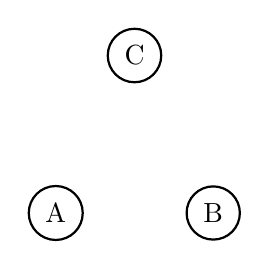
\begin{tikzpicture}
			\begin{scope}[every node/.style={circle,thick,draw}]
				\node (A) at (0,0) {A};
				\node (B) at (2,0) {B};
				\node (C) at (1,2) {C};
			\end{scope}
			
			\begin{scope}
				%\path (A) edge node {} (B);
				%\path (B) edge node {} (C);
				%\path (C) edge node {} (A);
			\end{scope}
		\end{tikzpicture}
		\caption{003 configuration}
	\end{subfigure}
	\hfill
	\begin{subfigure}[b]{0.2\linewidth}
		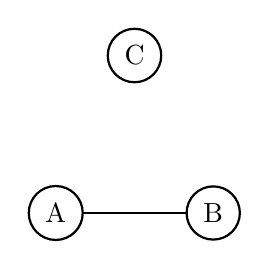
\begin{tikzpicture}
			\begin{scope}[every node/.style={circle,thick,draw}]
				\node (A) at (0,0) {A};
				\node (B) at (2,0) {B};
				\node (C) at (1,2) {C};
			\end{scope}
			
			\begin{scope}
				\path (A) edge node {} (B);
				%\path (B) edge node {} (C);
				%\path (C) edge node {} (A);
			\end{scope}
		\end{tikzpicture}
		\caption{102 configuration}
	\end{subfigure}
	\hfill
	\begin{subfigure}[b]{0.2\linewidth}
		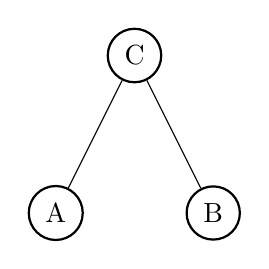
\begin{tikzpicture}
			\begin{scope}[every node/.style={circle,thick,draw}]
				\node (A) at (0,0) {A};
				\node (B) at (2,0) {B};
				\node (C) at (1,2) {C};
			\end{scope}
			
			\begin{scope}
				%\path (A) edge node {} (B);
				\path (B) edge node {} (C);
				\path (C) edge node {} (A);
			\end{scope}
		\end{tikzpicture}
		\caption{201 configuration}
	\end{subfigure}
	\hfill
	\begin{subfigure}[b]{0.2\linewidth}
		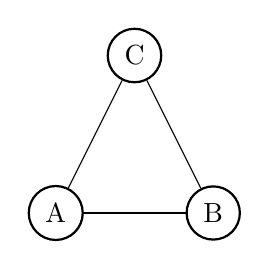
\begin{tikzpicture}
			\begin{scope}[every node/.style={circle,thick,draw}]
				\node (A) at (0,0) {A};
				\node (B) at (2,0) {B};
				\node (C) at (1,2) {C};
			\end{scope}
			
			\begin{scope}
				\path (A) edge node {} (B);
				\path (B) edge node {} (C);
				\path (C) edge node {} (A);
			\end{scope}
		\end{tikzpicture}
		\caption{300 configuration}
	\end{subfigure}
	\label{fig:triadic_structures}
	\caption{Possible triadic structures for any three nodes $A,B,C$.}
\end{figure}


\section{China Dataset}
\label{sec:china_data}

This dataset contains COVID case information from all of China \cite{china_publication,china_data}. There are 26961 entries (subject to change, depending on possible further preprocessing), with dates ranging from 2020-01-01 to 2022-08-14; therefore, this set stretches over most of the pandemic (as of writing this). Relevant covariates are listed in table \ref{tab:china_covariates}. In contrast to the former datasets, this one contains quite a few more that might yield interesting insights into infection dynamics. 2012 cases have no tie at all, 6179 have one tie, 12818 have two ties, 3194 have three ties, 1619 have four ties, 966 have five ties, 504 have six ties and 2237 cases have more than six ties. 1333 out of 3573 connected components are comprised of more than three nodes. An average degree of $3.6\pm18$, a median degree of 2 and only 2012 cases with no ties mean this network is significantly denser compared to the ones discussed previously. The mean age of patients is $42\pm18$, the 25 percentile is 30, the median is 41 and the 75 percentile is 54, meaning this dataset contains members of all age groups. There is no information on age for 6915 cases. 9218 women versus 11414 men shows a slight bias towards men; 6329 entries contain no information on sex. The three most common occupations are \emph{student} (970), \emph{worker} (548) and \emph{employee} (326). The three most common places of residence are \emph{Xi'an in Shanxi} (1984), \emph{Wuhan in Hubei} (1715) and \emph{Shijiazhuang in Hebei} (888). Where information was recorded, 462 cases have the Delta and 139 cases the Omicron variant. Among the most common activities suspected to be linked to the infection are \emph{travel to Wuhan} (635), \emph{dinner} (359) and \emph{residence in Wuhan} (337). Infections mostly happened during a family gathering (938), outdoors (791) and in a social setting (503). Sources of infection include confirmed cases, family members and \emph{Wuhan personnel}.

\section{Bucharest Dataset}
\label{sec:bucharest_dataset}

This dataset contains COVID case information from Bucharest, the capital of Romania. It consists of 46,269 positively tested patients, of which 6,895 named at least one other person as a possible contact. Out of the 13,272 individuals nominated as contacts, 1,811 were themselves recorded as patients; therefore, this dataset differs from the others in the sense that not all named contacts were tested positive. Dates range from 2020-03-07 to 2020-11-11. Patient covariates deemed relevant are age, sex, the patient's field of work and whether the patient is active in the medical field. 38,122 patients have nominated no one as contact, 15,856 have nominated one contact, 2,130 have nominated two contacts, and 1727 patients have named three or more persons as contacts. 
The average age of cases is $41\pm19$, with a 25 percentile of 29 and a 75 percentile of 53, meaning most are on the younger side. 21,655 males versus 24,604 females shows a slight bias towards females. Of the 6,964 patients where this information was recorded, only 186 are active in the medical field. Furthermore, a majority of patients for whom job information was recorded are not active in the labour market (6,298 out of 9,806). 

\paragraph{A note on data availability and ethical considerations} Although a fair number of research on the topic of contact tracing data have been published (e.g. \add{CITE}), general data availability was rather restricted at the time of writing this. Many datasets were either only available upon request to the respective author or outright unavailable, presumably due to privacy considerations. Some were even behind paywalls. Due to this, four of the five datasets used in this work originate from China, where such data is widely available and was regularly published by local health authorities during the pandemic. Since all data records have been pseudonymised, there should be no ethical concern regarding privacy violation.
	\chapter{Methodology}
\label{ch:methods}
	\chapter{Results and Discussion}
\label{ch:results_discussion}
	\chapter{5\quad Outlook}

In hindsight, it would have made more sense to identify cliques instead of connected components.
	\listoffigures
	\listoftables
	\printbibliography
\end{document}